\documentclass{beamer}
\usepackage{pgfpages}
\usepackage{xcolor}
\usepackage{graphicx}
\usepackage{caption}
\usepackage{hyperref}

\usetheme[sectionpage=simple,block=fill]{metropolis}
% \setbeameroption{show notes on second screen}

\definecolor{ured}{HTML}{CC0000}
\definecolor{ugray}{HTML}{808080}
\setbeamercolor{title separator}{fg=ured}
\setbeamercolor{frametitle}{bg=ured}

\title{Introduction to Automating System Builds, Workflows, and Configuration Management with GitHub Actions}
\date{June 29, 2021}
\author{Emerson Ford}
\institute{University of Utah --- ITX Meeting}

\begin{document}
\maketitle

\begin{frame}{Hello world!}
    foobar

    --
\end{frame}

\begin{frame}{Overview}
    \begin{itemize}
        \item Understanding automation
        \item How to automate with Github Actions
        \item Best practices of automation
        \item Q\&A and related topics
    \end{itemize}
\end{frame}

\begin{frame}{What is automation?}
    Getting computers do things for you automatically
    \begin{itemize}
        \item building, testing, and publishing artifacts
        \item linting and auto formatting code
        \item deploying configurations
        \item welcome new contributors to your repo \begin{minipage}{\linewidth}\vspace{2pt}
\includegraphics[width=0.8\linewidth]{welcome.png}\end{minipage}
    \end{itemize}
\end{frame}

\begin{frame}{Why automate?}
    \begin{itemize}
        \item saves you time and headaches
        \item ensure consistent workflow runs
        \item improve visiblity, handoff, and usability
        \item provides possible revert / rollback functionality
        \item it scales
    \end{itemize}
\end{frame}

\begin{frame}[plain]
    \begin{minipage}{\textwidth}
        \centering
        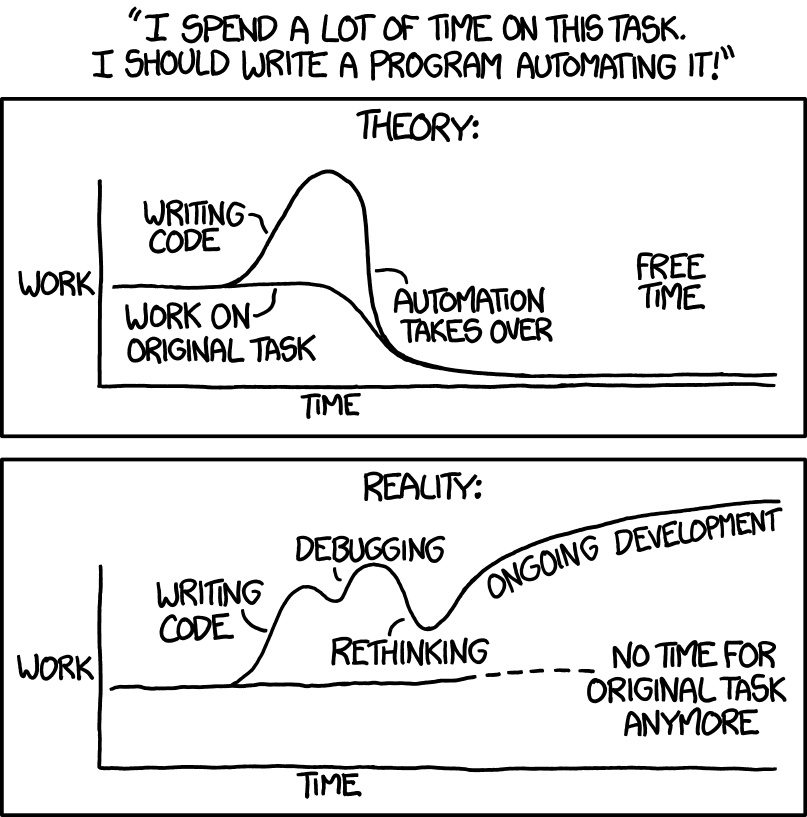
\includegraphics[width=0.7\linewidth]{automation_2x.png}
    \end{minipage}
\end{frame}

\begin{frame}[plain]
    \begin{minipage}{\textwidth}
        \centering
        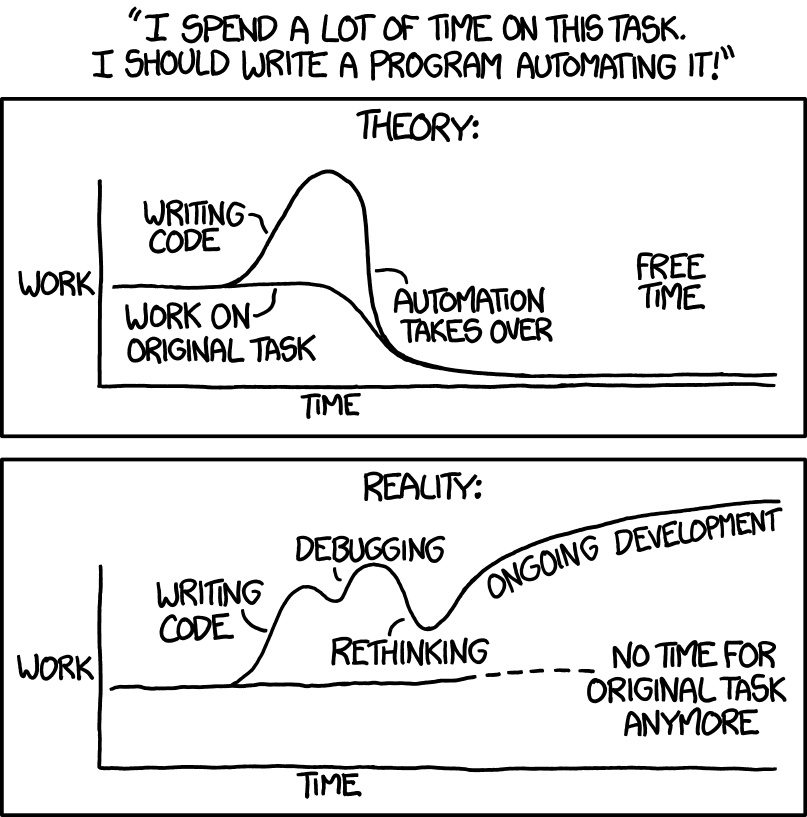
\includegraphics[width=0.4\linewidth]{automation_2x.png}
        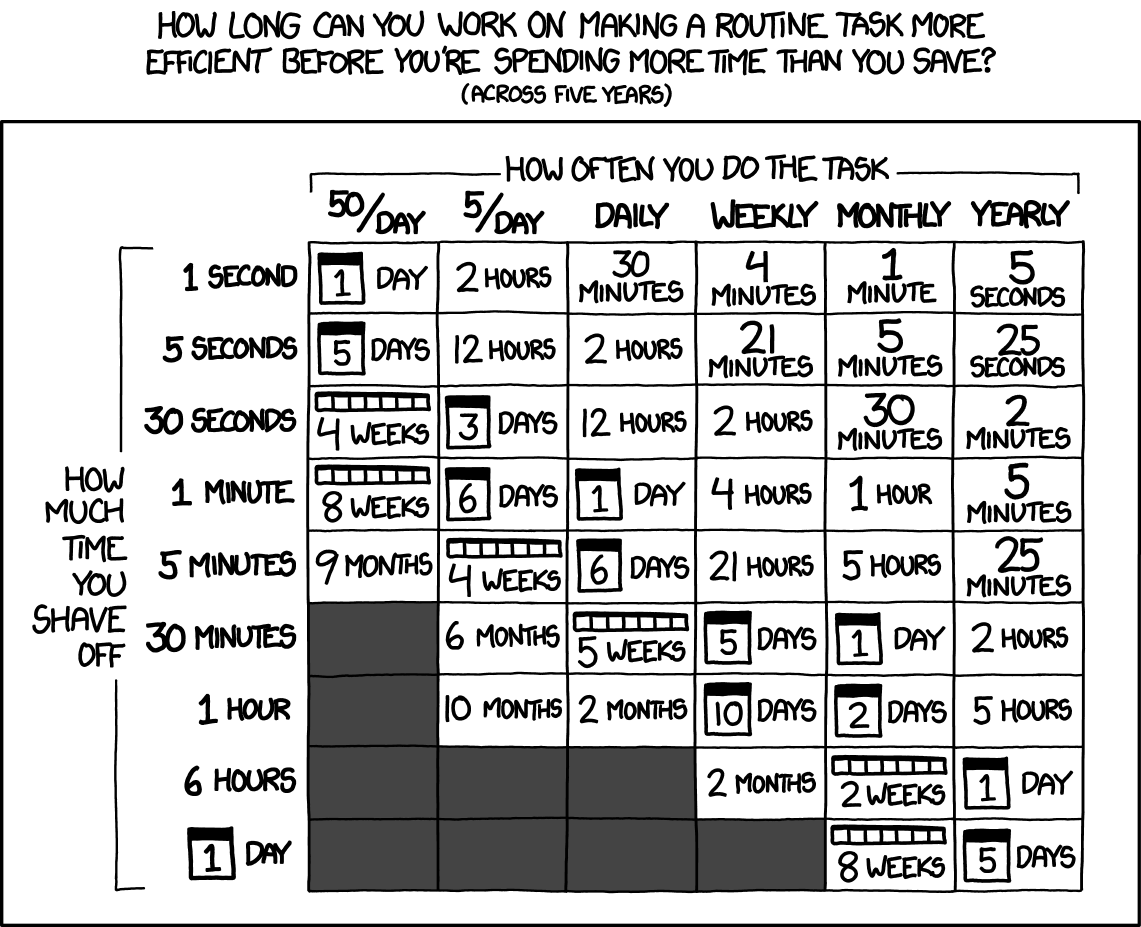
\includegraphics[width=0.5\linewidth]{is_it_worth_the_time_2x.png}
    \end{minipage}
\end{frame}

\begin{frame}[plain]
    \begin{minipage}{\textwidth}
        \centering
        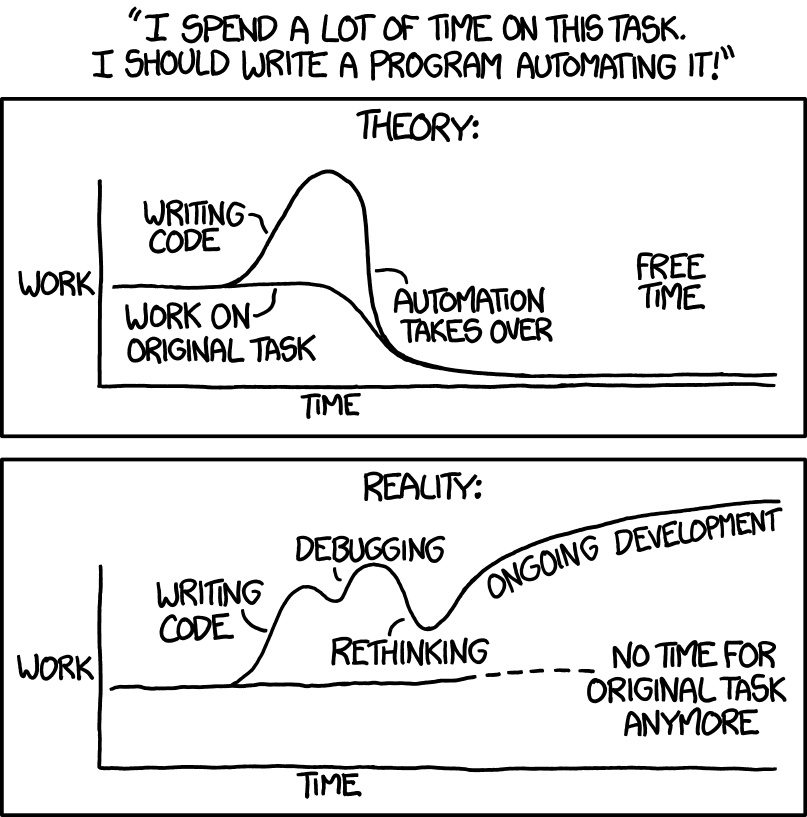
\includegraphics[width=0.4\linewidth]{automation_2x.png}
        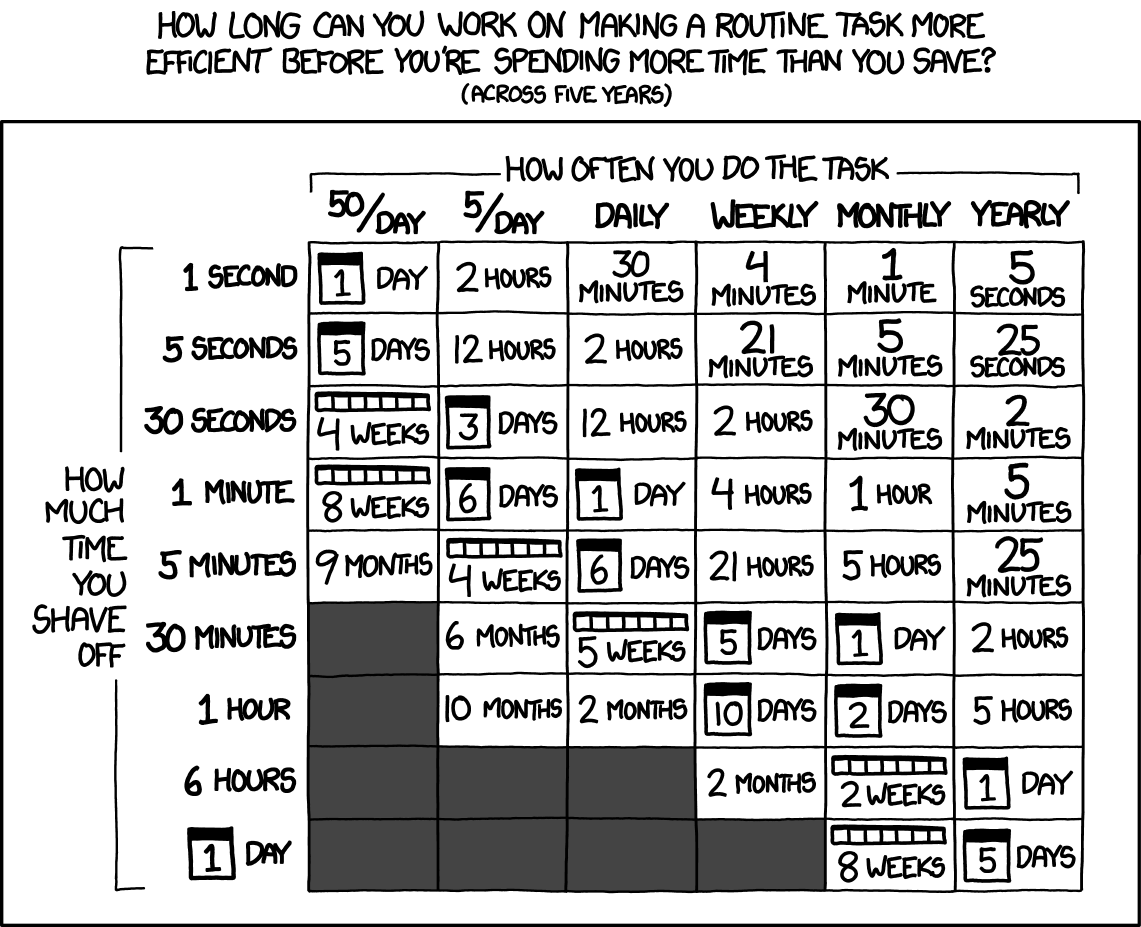
\includegraphics[width=0.5\linewidth]{is_it_worth_the_time_2x.png}
        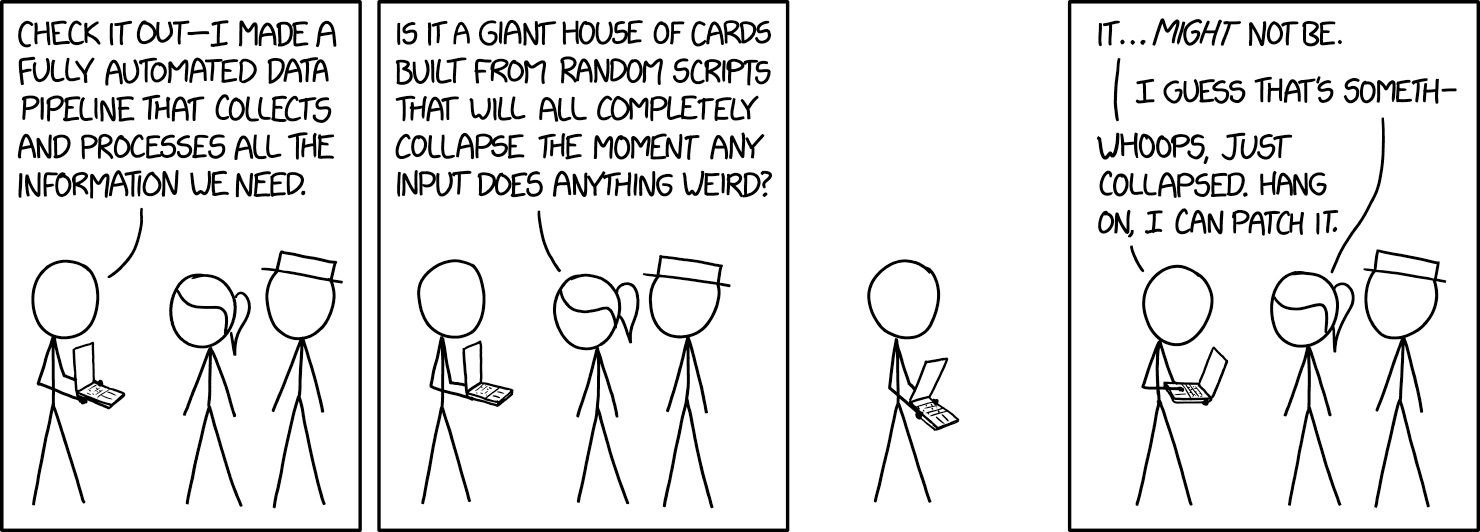
\includegraphics[width=0.47\linewidth]{data_pipeline_2x.png}
        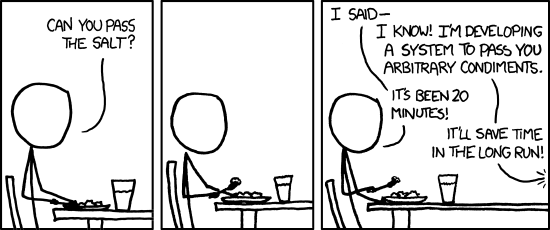
\includegraphics[width=0.4\linewidth]{the_general_problem.png}
        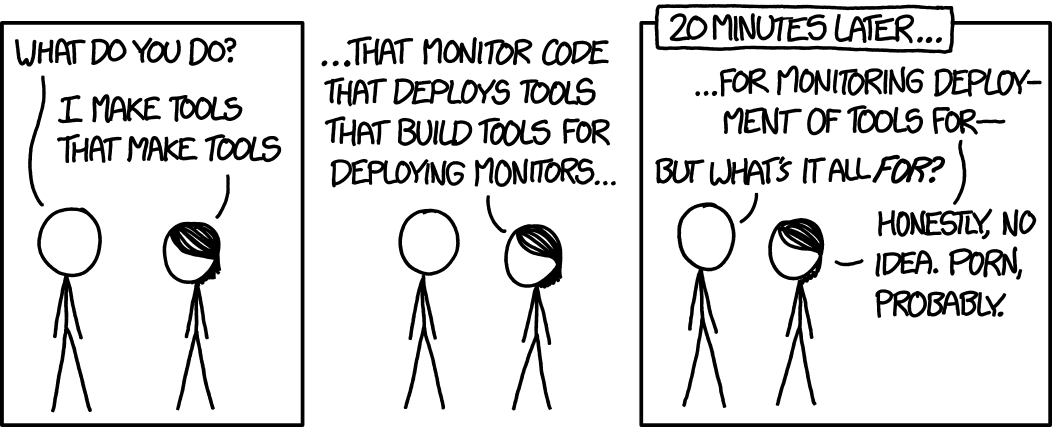
\includegraphics[width=0.4\linewidth]{tools_2x.png}
        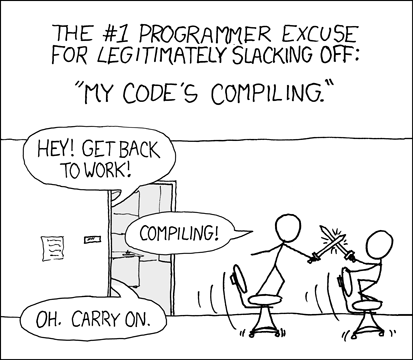
\includegraphics[width=0.2\linewidth]{compiling.png}
    \end{minipage}
\end{frame}


\section{How to Automate}

\begin{frame}{Github Actions}
    \begin{itemize}
        \item free product from Github for public repos
        \item ``on-demand'' VMs / containers
        \item triggered from git actions (push, pull request, etc)
        \item executions steps described in yaml
    \end{itemize}

    See \url{https://docs.github.com/en/actions/guides} for more information.
\end{frame}

\begin{frame}[plain]
    \begin{minipage}{\textwidth}
        \centering
        \only<1>{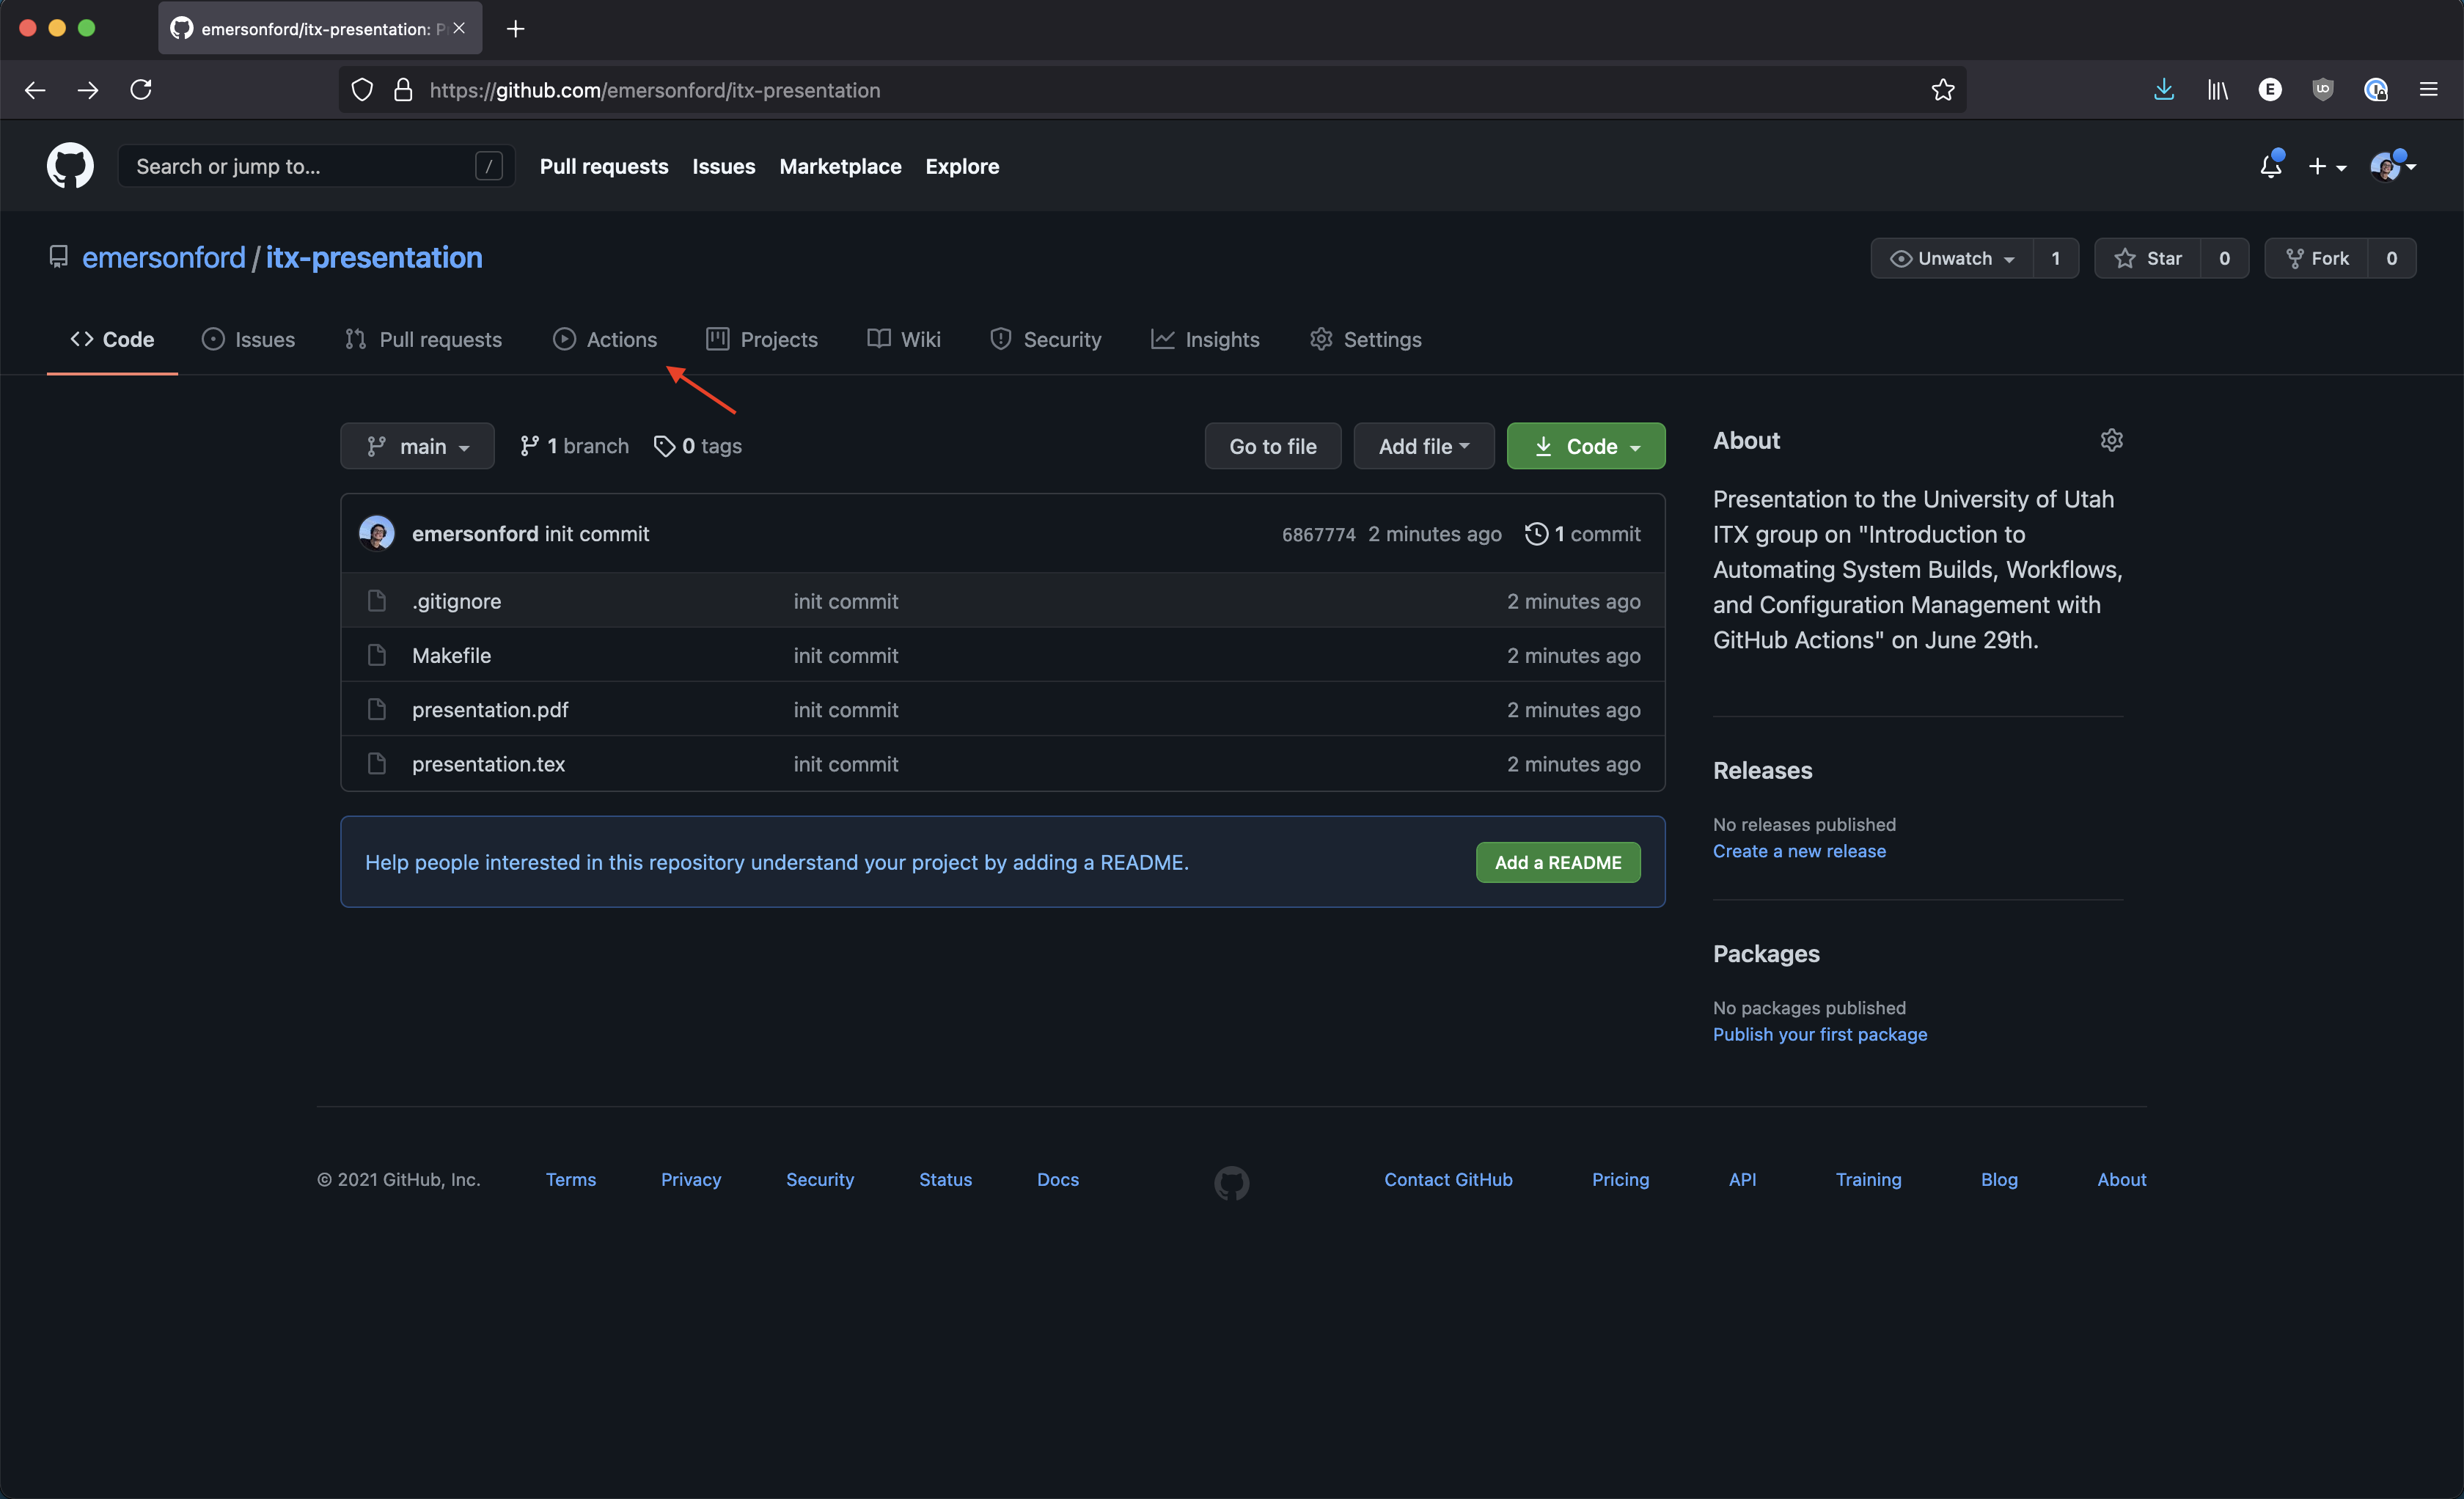
\includegraphics[width=\textwidth]{actions-getting-started1.png}}
        \only<2>{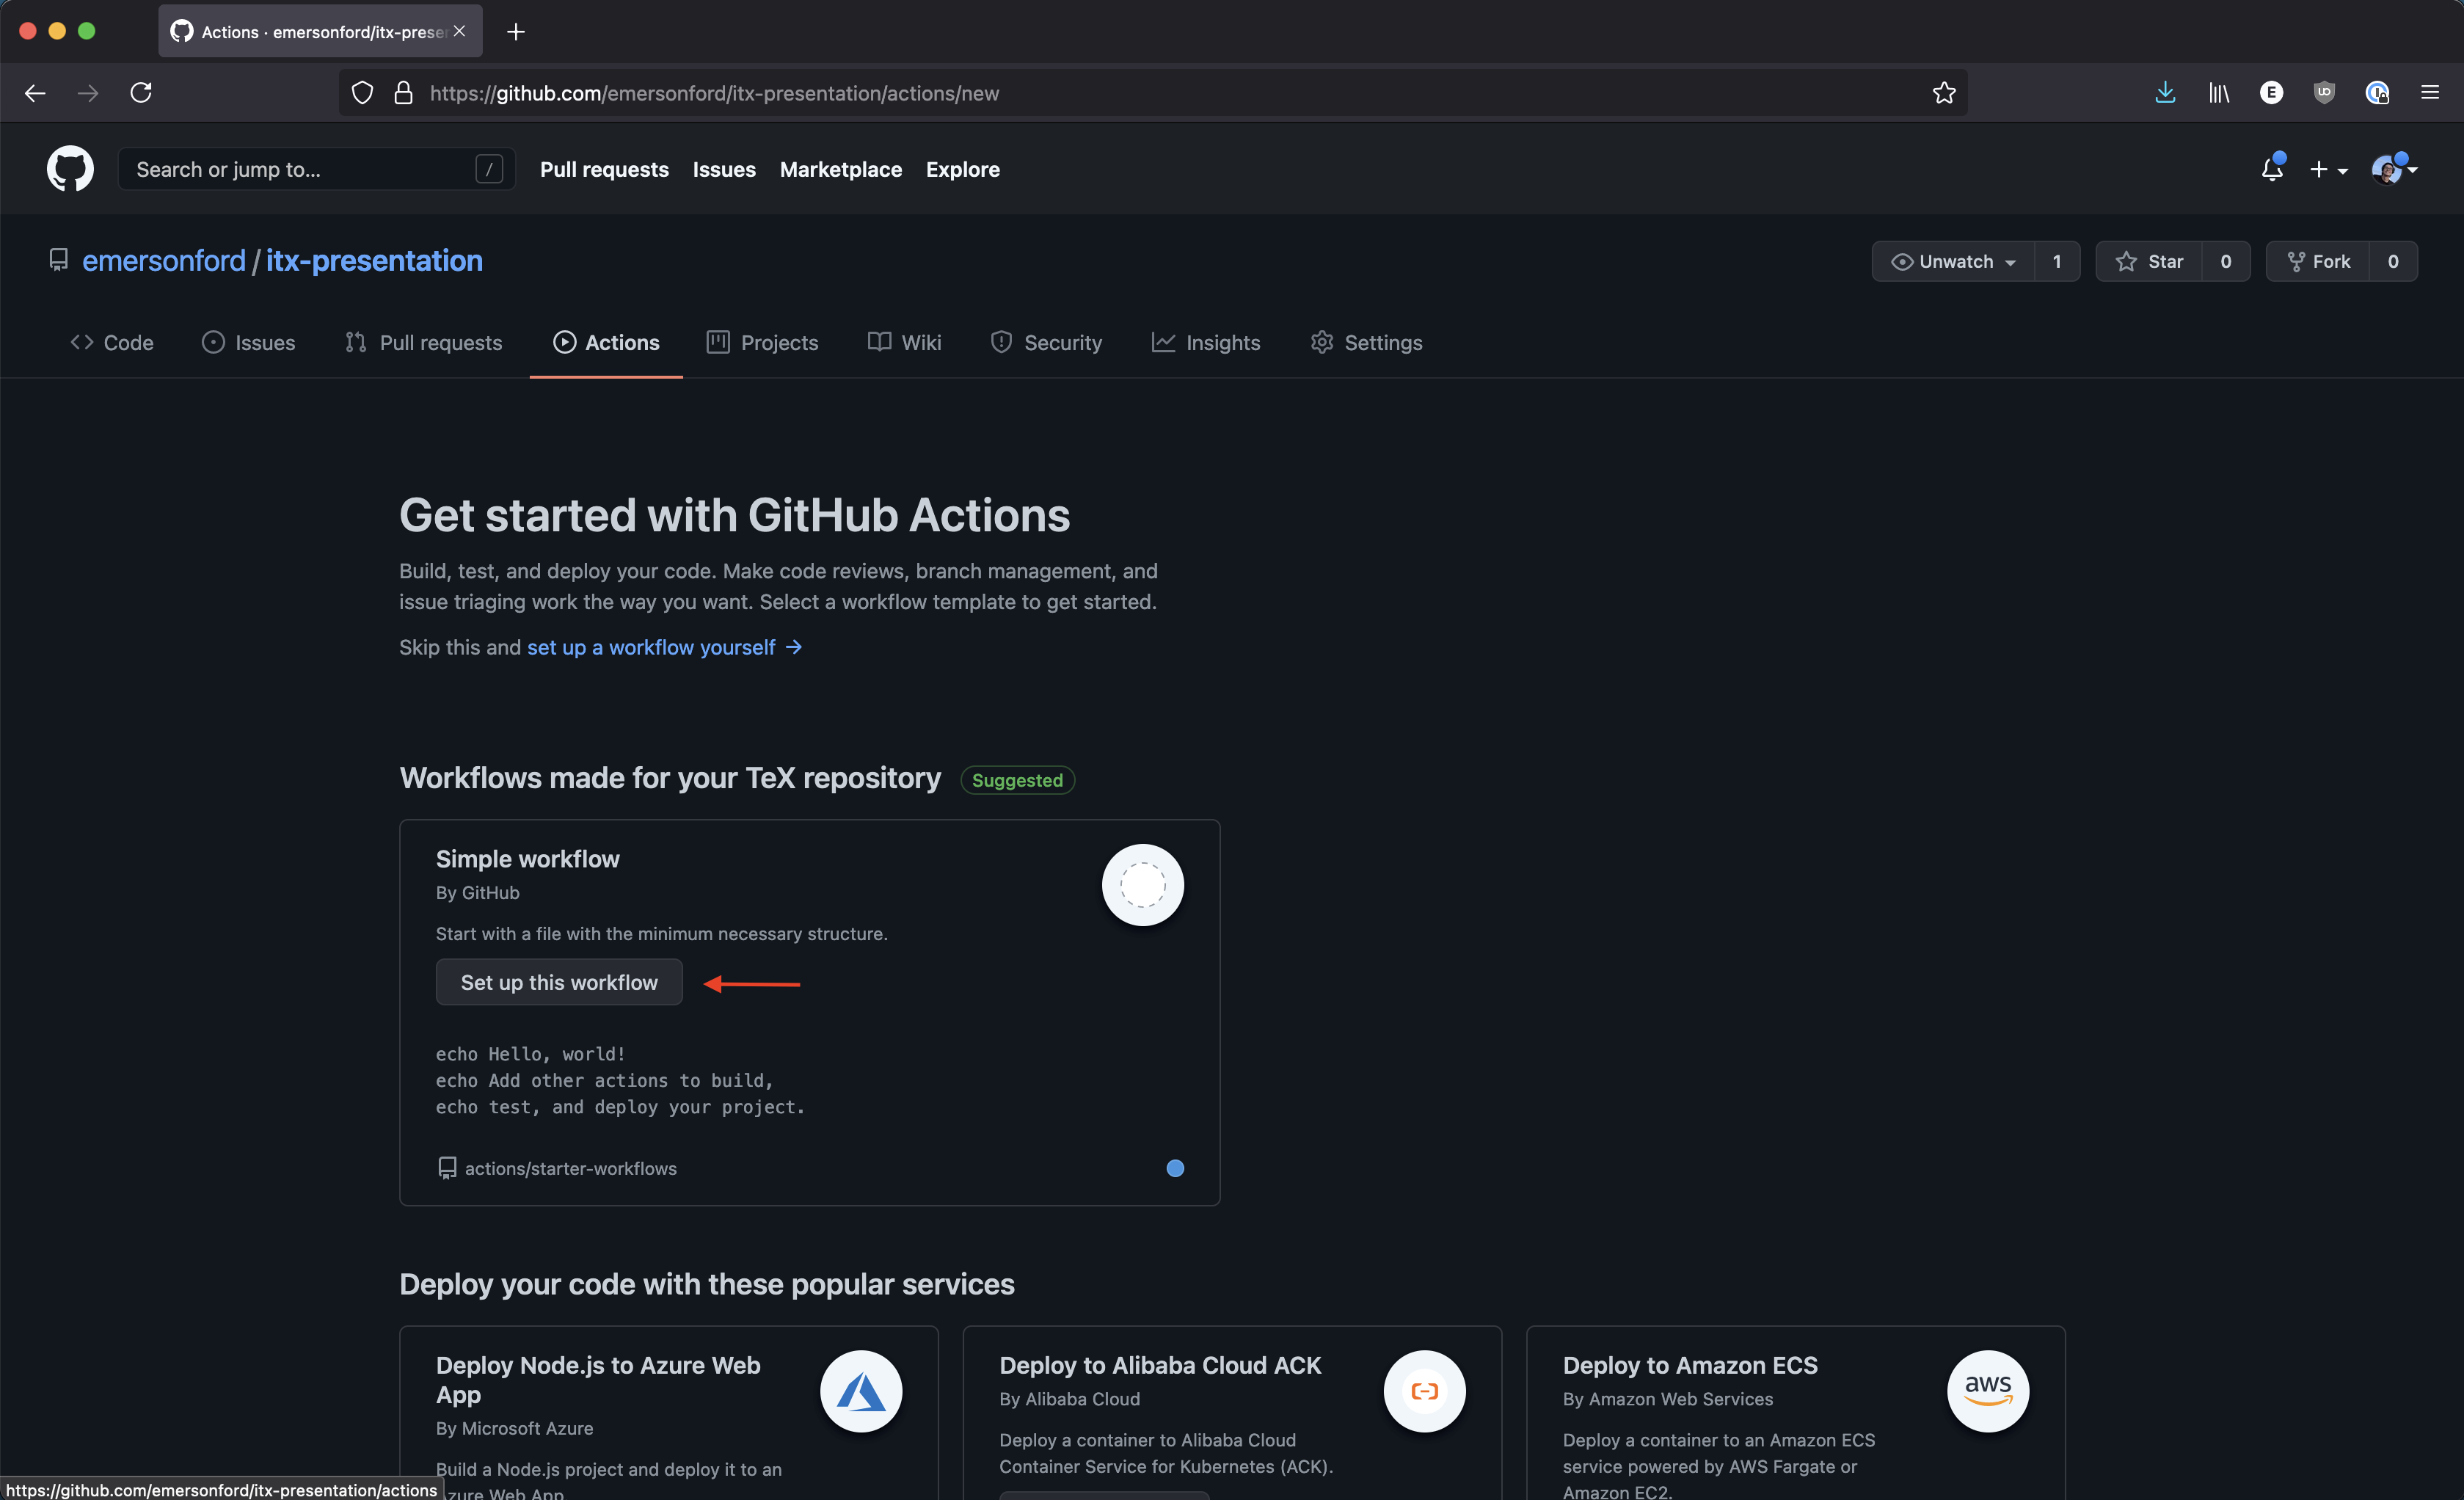
\includegraphics[width=\textwidth]{actions-getting-started2.png}}
        \only<3>{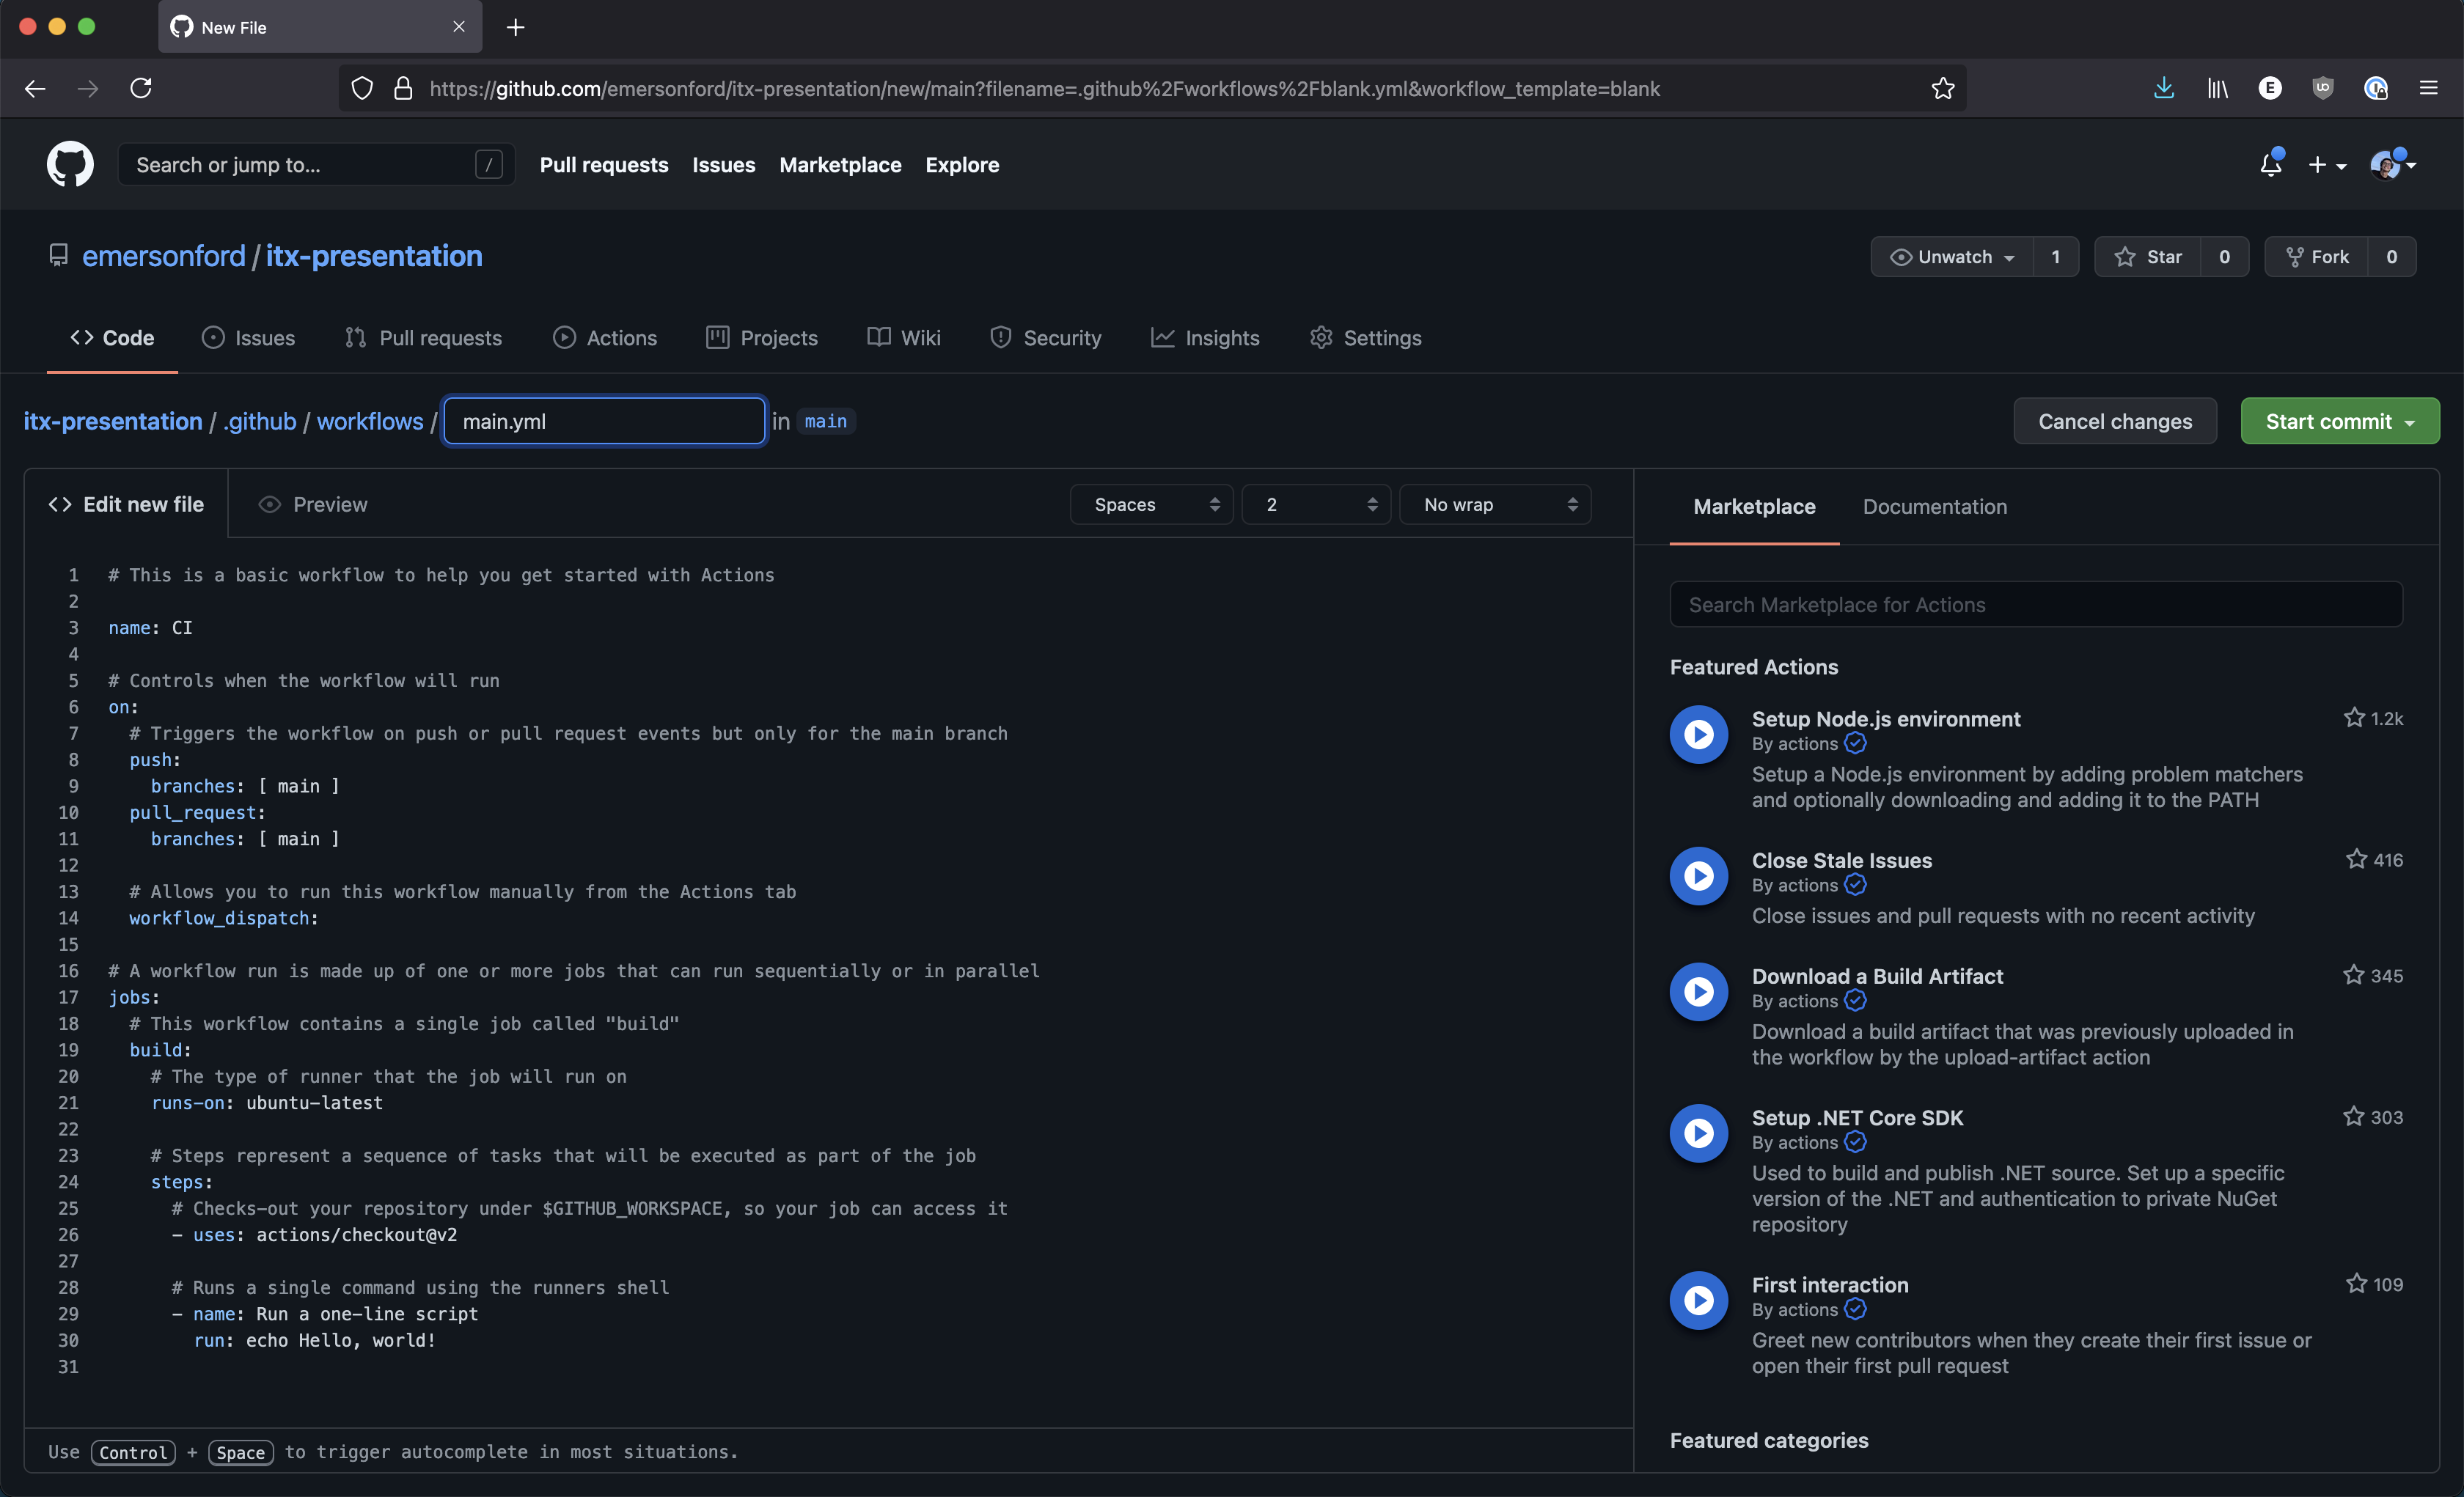
\includegraphics[width=\textwidth]{actions-getting-started3.png}}
    \end{minipage}
\end{frame}

\begin{frame}{Other Examples}
    \begin{itemize}
        \item deploy and configure infrastructure in the cloud
        \item build, security test, and publish container images
        \item do something when you comment on an issue
    \end{itemize}
\end{frame}

\begin{frame}{Best Practices}
    \begin{itemize}
        \item don't run actions on arbitrary pull requests
        \item pick a model for how to use Git and stick with it (rebase only, git-flow, etc)
        \item don't let developers shoot themselves in the foot
    \end{itemize}
\end{frame}

\section{Questions?}

\begin{frame}{Related Topics}
    \begin{itemize}
        \item Declarative Infrastructure Management
            \begin{itemize}
                \item Terraform for Cloud Deployment
                \item Ansible for Node Configuration
            \end{itemize}
        \item GitOps
        \item Applying CI/CD to containers and Kubernetes
        \item Secrets management in Git repos
        \item Best practices / understanding Git
        \item Alternative CI/CD solutions such as Gitlab Runners, Jenkins, CircleCI, etc.
    \end{itemize}
\end{frame}

\begin{frame}{Link}
    \url{https://github.com/emersonford/itx-presentation}
\end{frame}



\end{document}
